\chapter{Números/Relações (4º Bimestre)}

\section{Gráficos e tabelas}

\subsection*{Exercício 1}

According to an estimativa populacional do Instituto Brasileiro de Geografia e
Estatística (IBGE) para 1º de julho de 2014, the 10 aglomerados urbanos mais
populosos do Brasil are given by the following table

\begin{center}
  \begin{tabular}{ l | l}    \hline
Localidade      & Pop.      \\ \hline
São Paulo 	&20 935 204 \\ \hline
Rio de Janeiro 	&12 116 616 \\ \hline
Belo Horizonte 	&5 783 773 \\ \hline
Porto Alegre 	&4 181 836 \\ \hline
Brasília 	&4 118 154 \\ \hline
Salvador 	&3 919 864 \\ \hline
Recife 	 	&3 887 261 \\ \hline
Fortaleza 	&3 818 380 \\ \hline
Curitiba 	&3 466 981 \\ \hline
Campinas 	&3 043 217 \\
    \hline
  \end{tabular}
\end{center}

Represent this statistic table as a diagram of bars, for which a length of
${1\text{cm}}$ represents $2000000$ inhabitants. Indicate some benefits of
this representation.

\subsection*{Exercício 2}

A poll Ibope from the 7 to 8 October 2014 was realized on 3010 people
regarding the segundo turno do Eleição presidencial no Brasil. 1324 people
indicated they will vote for Dilma Rousseff, 1385 people indicated they
will vote for Aécio Neves, 181 people indicated they will vote Branco / Nulo
and the remaining people didn't indicate their intention to vote.

\begin{enumerate}
\item Draw a pie chart representing the result of this poll.
\item Dilma Rousseff won the election with $51.64\%$ votes. Compare
  with your diagram. How can you explain this difference?
\end{enumerate}

\section{Medidas de tendência central}

\subsection*{Definición}

Consideramos $n$ datos $x_1, x_2, \ldots, x_n$. La media (aritmética) de esos
valores es
%%
$$\mu = E(x) =
\overline{x} = \frac{x_1 + x_2 + \ldots + x_n}{n} = \frac{1}{n}\sum_{i=1}^n x_i$$

La moda es el valor lo más repetido en estos datos. Es posible que no sea
única.

Si ordenados las valores
de menor a mayor, la mediana es el valor de la variable a la mitad de los datos
(si hay un número impar de datos)
o la media de las valores dos variables a la mitad (si hay un número par de
datos).

\subsection*{Ejemplo}

Consideramos los datos $x_1 = x_4 = x_5 = 3$, $x_2 = x_6 = 1$,
$x_3 = 0$ y $x_7 = 10$. La media es $\frac{3+1+0+3+3+1+10}{7} = 3$. La moda
es $3$, valor tomado por $x_1, x_4, x_5$. Podemos ordenar las variables:
$x_3 = 0, 1, 1, {\color{red}3}, 3, 3, 10 = x_7$ y entonces la mediana es también $3$.

Ahora, añadimos el dato $x_8 = 1$. La media se vuelve
$\frac{3+1+0+3+3+1+10+1}{8} = 2.75$. Hay dos modas de frecuencia $3$ posibles:
$3$ (valor tomado por $x_1, x_4, x_5$) y
$1$ (valor tomado por $x_2, x_6, x_8$). Podemos ordenar las variables:
$x_3 = 0, 1, 1, {\color{red} 1}, {\color{red} 3}, 3, 3, 10 = x_7$ y entonces
la mediana es $\frac{1+3}{2} = 2$.

\subsection*{Exercício 3}

Calcule la media, moda y mediana de estos datos

\begin{enumerate}
\item $1.60\text{m}, 1.58\text{m}, 1.66\text{m}, 1.72\text{m}, 1.67\text{m}, 1.73\text{m}, 1.65\text{m}, 1.66\text{m}, 1.70\text{m}, 1.80\text{m}$
\item $18 \text{años}, 25 \text{años}, 22 \text{años},  \text{22} \text{años},
   \text{22} \text{años},  \text{18} \text{años},
   \text{24} \text{años},  \text{20} \text{años},  \text{29} \text{años}$
\end{enumerate}

\section*{Problemas de contagem}

La probabilidad $p$ de que suceda un evento $A$ de un total de $n$ casos
posibles igualmente probables es igual a la razón entre el número de
ocurrencias $k$ de dicho evento (casos favorables) y el número total de casos
posibles $n$.

$$
p=P\left(A\right)=\frac {k}{n}
$$

The probability that the event does not happen (denoted by $\bar{A}$) is then
%%
$$
1-p=P\left(\bar{A}\right)= \frac {n - k}{n}
$$

\subsection*{Ejercicio 4}

En una baraja de 52 naipes, cual es la probabilidad de tirar:

\begin{enumerate}
\item El siete de diamantes.
\item Un rey.
\item Una carta de picas.
\item Una figura (As, rey, reina o paje).
\item Un número par.
\end{enumerate}

\subsection*{Exercício 5}

A bag contains three red balls, two blue balls and four green ball. We pick
one ball randomly from the bag:

\begin{enumerate}
\item What is the total number of balls?
\item What is the probability to pick a red ball? a blue one? a green one?
\end{enumerate}

We now consider two events $A$, $B$. The number of cases when $A$ happens is
still $k$, over a total of $n$ possibilities. Among these $0 \leq k \leq n$
cases, we suppose that the number of cases when $B$ happens is
$0 \leq l \leq k$.

As above, we can define the probability
that $A$ happens $P{(A)} = \frac{k}{n}$ ($k$ cases over $n$) and the
probability that both $A$ and $B$ happen
$P{(A \text{e} B)} = \frac{l}{n}$ ($l$ cases over $n$).

Assuming that $A$ happens ($k$ cases), there are $l$ cases when $B$ happens,
that is a probability $P{(B|A)} = \frac{l}{k}$ (``$B$ knowing $A$''). As
a consequence we find the product rule:

$$P{(A \text{e} B)} = \frac{l}{n} = {\frac{k}{n} \frac{l}{k}} =
{P{(A)} \times P{(B|A)}}$$

We can then define similar probabilities for $\bar{B}$ and $\bar{A}$. We finally
can summarize everything in a diagrama de árvore:

\begin{center}
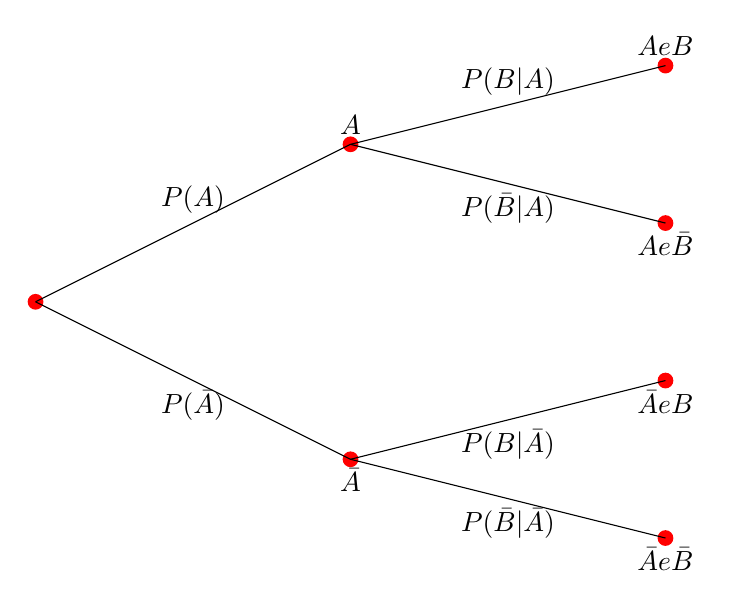
\begin{tikzpicture}
  \path[fill=red](0,0) circle(.1);
  \path[fill=red](4,2) circle(.1);
  \path[fill=red](4,-2) circle(.1);
  \path[fill=red](8,3) circle(.1);
  \path[fill=red](8,-3) circle(.1);
  \path[fill=red](8,1) circle(.1);
  \path[fill=red](8,-1) circle(.1);
  \draw (0,0) -- (2,1) node[above]{$P(A)$} -- (4,2) node[above]{$A$} --
  (6,2.5) node[above]{$P(B|A)$} -- (8,3) node[above]{$A \text{e} B$};
  \draw (0,0) -- (2,-1) node[below]{$P(\bar{A})$} -- (4,-2) node[below]{$\bar{A}$} -- (6,-2.5) node[below]{$P(\bar{B}|\bar{A})$} -- (8,-3) node[below]{$\bar{A} \text{e} \bar{B}$};
  \draw (4,2) -- (6,1.5) node[below]{$P(\bar{B}|A)$} -- (8,1) node[below]{$A \text{e} \bar{B}$};
  \draw (4,-2) -- (6,-1.5) node[below]{$P(B|\bar{A})$} -- (8,-1) node[below]{$\bar{A} \text{e} B$};
\end{tikzpicture}
\end{center}

\subsection*{Exercício 6}

In the exercise $4$, once we pick one ball we remove all the balls of the
same color from the bag. Then we pick a second ball randomly.
Let $A$ be the event ``the first ball is red'',
$B$ the event ``the second ball is blue''

\begin{enumerate}
\item Determine $P(A)$, $P(\bar{A})$.
\item Suppose that we first
  pick a red ball and so remove all the other red balls.
  How many balls remain? How many blue balls remain? 
  Deduce $P(B|A)$ and $P(\bar{B}|A)$.
\item Suppose that we first pick a green ball.
  How many possibililites are there for the second ball? Among them,
  in how many cases does $B$ happen?
\item Suppose that we first pick a blue ball.
  How many possibililites are there for the second ball? Among them,
  in how many cases does $B$ happen?
\item Deduce $P(B|\bar{A})$ and $P(\bar{B}|\bar{A})$.
\item Draw the diagrama de árvore, placing the probabilities determined above.
\item How to interpret the product rules on the diagram?
  Deduce the probabilities of
   $A \text{e} B$, $A \text{e} \bar{B}$, $\bar{A} \text{e} B$ and
  $\bar{A} \text{e} \bar{B}$,
\item What is $P(B)$?
\end{enumerate}

\section{Solução dos exercícios}

\subsection*{Exercício 1}

\begin{center}
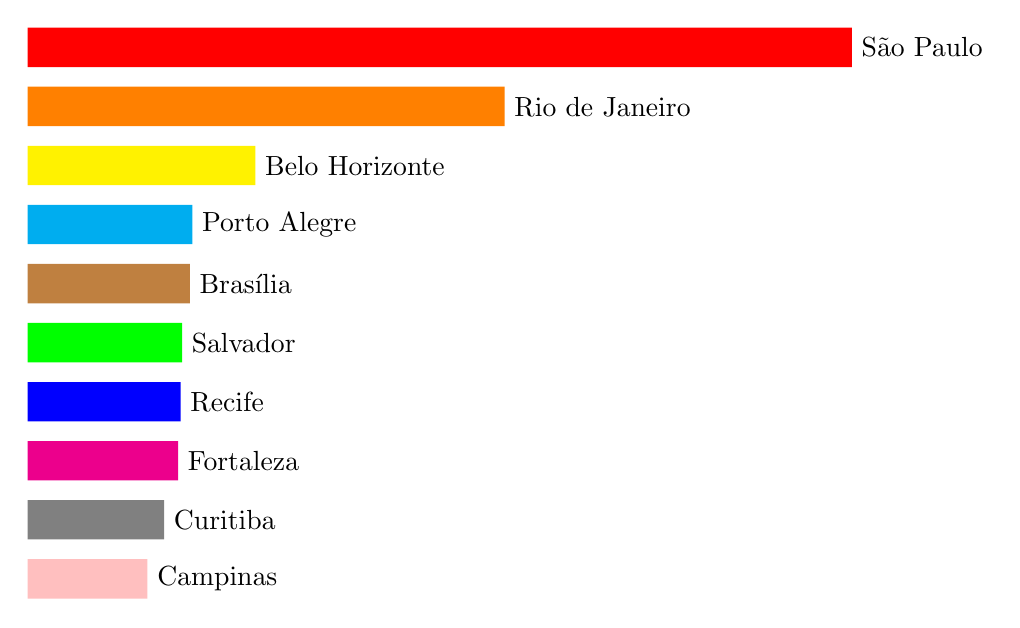
\begin{tikzpicture}[xscale=.5,yscale=-.5]
  \path[fill=red] (0,0) -- (20.935204,0) -- (20.935204,.5) node[right]{São Paulo} -- (20.935204,1) -- (0,1) -- cycle;
  \path[fill=orange] (0,1.5) -- (12.116616,1.5) -- (12.116616,2) node[right]{Rio de Janeiro} -- (12.116616,2.5) -- (0,2.5) -- cycle;
  \path[fill=yellow] (0,3) -- (5.783773,3) -- (5.783773,3.5) node[right]{Belo Horizonte} -- (5.783773,4) -- (0,4) -- cycle;
  \path[fill=cyan] (0,4.5) -- (4.181836,4.5) -- (4.181836,5) node[right]{Porto Alegre} -- (4.181836,5.5) -- (0,5.5) -- cycle;
  \path[fill=brown] (0,6) -- (4.118154,6) -- (4.118154,6.5) node[right]{Brasília} -- (4.118154,7) -- (0,7) -- cycle;
  \path[fill=green] (0,7.5) -- (3.919864,7.5) -- (3.919864,8) node[right]{Salvador} -- (3.919864,8.5) -- (0,8.5) -- cycle;
  \path[fill=blue] (0,9) -- (3.887261,9) -- (3.887261,9.5) node[right]{Recife} -- (3.887261,10) -- (0,10) -- cycle;
  \path[fill=magenta] (0,10.5) -- (3.818380,10.5) -- (3.818380,11) node[right]{Fortaleza} -- (3.818380,11.5) -- (0,11.5) -- cycle;
  \path[fill=gray] (0,12) -- (3.466981,12) -- (3.466981,12.5) node[right]{Curitiba} -- (3.466981,13) -- (0,13) -- cycle;
  \path[fill=pink] (0,13.5) -- (3.043217,13.5) -- (3.043217,14) node[right]{Campinas} -- (3.043217,14.5) -- (0,14.5) -- cycle;
\end{tikzpicture}
\end{center}

This representation allows for example to quickly compare the relative numbers
inhabitants visually.
For example that Rio de Janeiro as about four times as many inhabitants as
Campinas.

\subsection*{Exercício 2}

\begin{enumerate}

\item

  \begin{center}
    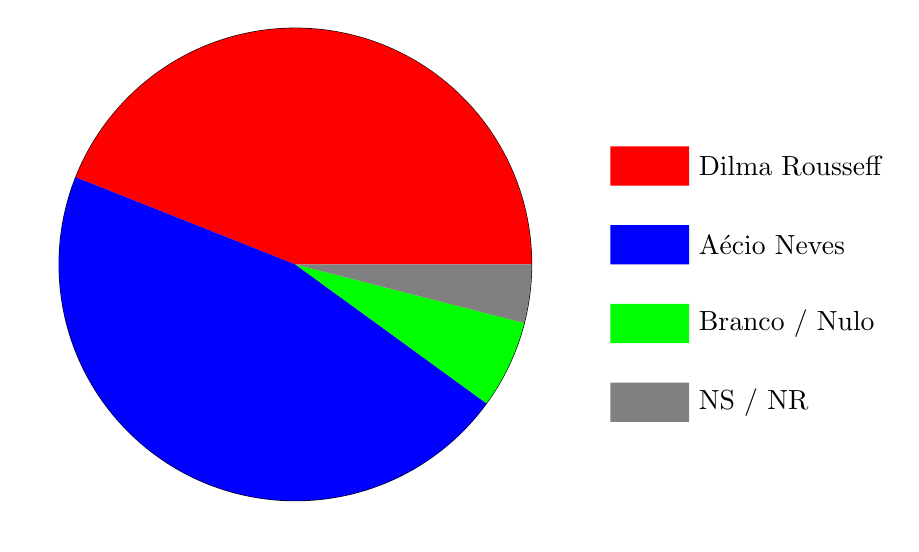
\begin{tikzpicture}
      \begin{scope}[shift={(4,1)}]
        \path[fill=red] (0,0) -- (1,0) -- (1,.25)node[right]{Dilma Rousseff} -- (1,.5) -- (0,.5) -- cycle;
      \end{scope}
      \begin{scope}[shift={(4,0)}]
        \path[fill=blue] (0,0) -- (1,0) -- (1,.25)node[right]{Aécio Neves} -- (1,.5) -- (0,.5) -- cycle;
      \end{scope}
      \begin{scope}[shift={(4,-1)}]
        \path[fill=green] (0,0) -- (1,0) -- (1,.25)node[right]{Branco / Nulo} -- (1,.5) -- (0,.5) -- cycle;
      \end{scope}
      \begin{scope}[shift={(4,-2)}]
        \path[fill=gray] (0,0) -- (1,0) -- (1,.25)node[right]{NS / NR} -- (1,.5) -- (0,.5) -- cycle;
      \end{scope}

      \draw (0,0) circle(3)[color=black];
      \path[fill=red] (0,0) -- (3,0) arc(0:158.3521594684385:3);
      \path[fill=blue] (0,0) -- (-2.788406361270516,1.106702292590976) arc(158.3521594684385:324:3);
      \path[fill=green] (0,0) -- (2.427050983124842,-1.76335575687742) arc(324:345.6478405315615:3);
      \path[fill=gray] (0,0) -- (2.906371419754301,-0.7436431741335125) arc(345.6478405315615:360:3);
   \end{tikzpicture}
  \end{center}

\item The poll only gave $44\%$ of votes for Dilma Rousseff.
  Besides the fact that people may not have made their final choice or
  may not want to tell it, the sample is not perfectly representative of
  the whole population.

\end{enumerate}

\subsection*{Exercício 3}

\begin{enumerate}
\item
La media es
$\frac{1.6+1.68+1.66+1.72+1.67+1.73+1.65+1.66+1.7+1.8}{10} = 1.687\text{m}$,
la moda $1.66\text{m}$ (dos veces) y la mediana
$\frac{1.68+1.67}{2} = 1.675\text{m}$.

\item
La media es $\frac{18+25+22+22+22+24+24+21+20}{9} = 22 \text{años}$.
La moda es $22 \text{años}$ (tres veces) y la mediana es tambíen $22 \text{años}$.

\end{enumerate}

\subsection*{Exercício 4}

Hay 52 eventos equiprobables corespondente a cada carta.

\begin{enumerate}
\item $\frac{1}{52}$ (un siete de diamantes)
\item $\frac{4}{52} = \frac{1}{13}$ (4 reyes)
\item $\frac{9 + 4}{52} = \frac{1}{4}$ (9 números de picas y 4 figuras de picas)
\item $\frac{4 \times 4}{52} = \frac{4}{13}$ (4 figuras de 4 palos)
\item $\frac{4 \times 5}{52} = \frac{5}{13}$ (números 2, 4, 6, 8 y 10 de 4 palos)
\end{enumerate}

\subsection*{Exercício 5}

\begin{enumerate}
\item $3+2+5=10$
\item $\frac{3}{10}$, $\frac{2}{10} = \frac{1}{5}$ and $\frac{5}{10} =
  \frac{1}{2}$
\end{enumerate}

\subsection*{Exercício 6}

\begin{enumerate}
\item $\frac{3}{10}$ and $1 - \frac{3}{10} = \frac{7}{10}$.

\item If $A$ happens, we remove the remaining red balls and it remains
  six balls (two blue balls and four green balls). The probability
  $P(B|A)$ to get a blue ball is then $\frac{2}{6} = \frac{1}{3}$.
  The probability $P(B|\bar{A})$ to get a green ball then
  $1 - \frac{1}{3} = \frac{2}{3}$.

\item We remove all the green balls so it remains $5$ balls
  ($3$ red and $2$ blue) and as many possibilities for the second balls.
  $B$ happens in two cases.

\item We remove all the blue balls so it remains $7$ balls
  ($3$ red and $4$ green) and as many possibilities for the second balls.
  $B$ never happens because it does not remain any blue ball!

\item When $\bar{A}$ happens, there are $7+5$ possibilities for the second
  balls and among them, $B$ happens in two cases.
  So $P(B|\bar{A}) = \frac{2}{12} = \frac{1}{6}$ and
  $P(\bar{B}|\bar{A}) = 1 - \frac{1}{6} = \frac{5}{6}$.

\begin{center}
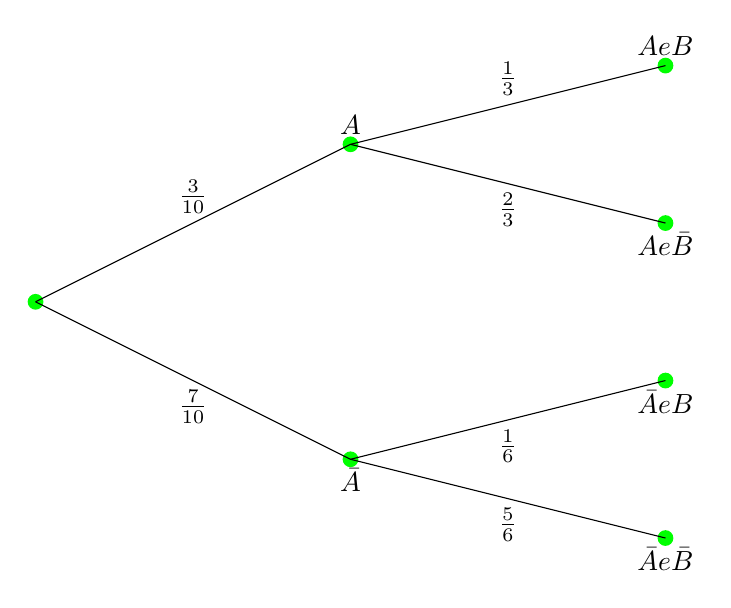
\begin{tikzpicture}
  \path[fill=green](0,0) circle(.1);
  \path[fill=green](4,2) circle(.1);
  \path[fill=green](4,-2) circle(.1);
  \path[fill=green](8,3) circle(.1);
  \path[fill=green](8,-3) circle(.1);
  \path[fill=green](8,1) circle(.1);
  \path[fill=green](8,-1) circle(.1);
  \draw (0,0) -- (2,1) node[above]{$\frac{3}{10}$} -- (4,2) node[above]{$A$} --
  (6,2.5) node[above]{$\frac{1}{3}$} -- (8,3) node[above]{$A \text{e} B$};
  \draw (0,0) -- (2,-1) node[below]{$\frac{7}{10}$} -- (4,-2) node[below]{$\bar{A}$} -- (6,-2.5) node[below]{$\frac{5}{6}$} -- (8,-3) node[below]{$\bar{A} \text{e} \bar{B}$};
  \draw (4,2) -- (6,1.5) node[below]{$\frac{2}{3}$} -- (8,1) node[below]{$A \text{e} \bar{B}$};
  \draw (4,-2) -- (6,-1.5) node[below]{$\frac{1}{6}$} -- (8,-1) node[below]{$\bar{A} \text{e} B$};
\end{tikzpicture}
\end{center}

\item To get the probabilities on the leaves
  $A \text{e} B$, $A \text{e} \bar{B}$, $\bar{A} \text{e} B$ and
  $\bar{A} \text{e} \bar{B}$,
  we follow the path from the root to a given leave and take the produce of
  the probabilities we find on the path. We get
  $\frac{3}{10} \times \frac{1}{3}= \frac{1}{10}$,
  $\frac{3}{10} \times \frac{2}{3} = \frac{1}{5}$,
  $\frac{7}{10} \times \frac{1}{6} = \frac{7}{60}$ and
  $\frac{7}{10} \times \frac{5}{6} = \frac{7}{12}$.

\item ${P(B)} = {P(\bar{A} \text{e} B)} +
  {P(A \text{e} B)} =  \frac{1}{10} + \frac{7}{60} = \frac{13}{60}$

\end{enumerate}

